

\tikzset{every picture/.style={line width=0.75pt}} %set default line width to 0.75pt        

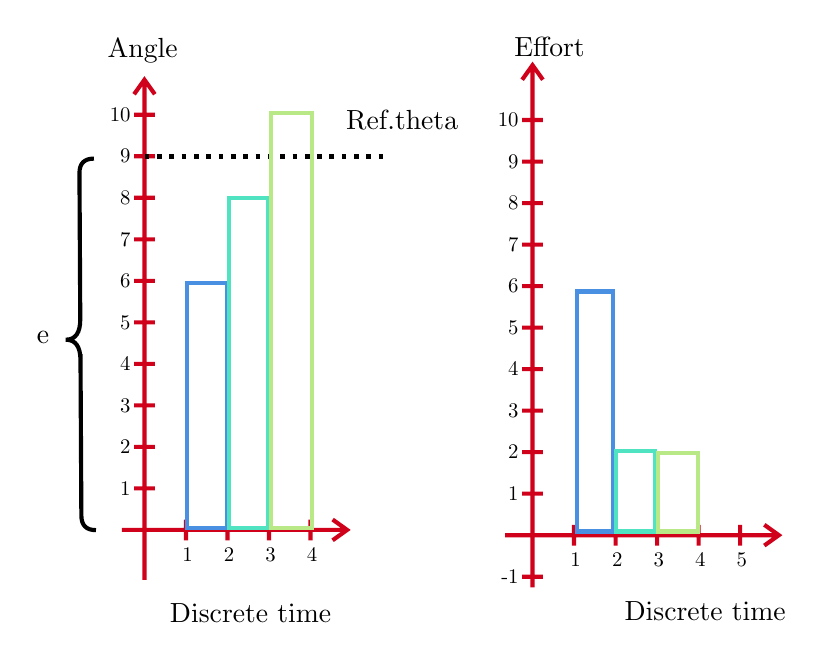
\begin{tikzpicture}[x=0.75pt,y=0.75pt,yscale=-1,xscale=1]
%uncomment if require: \path (0,530); %set diagram left start at 0, and has height of 530

%Shape: Axis 2D [id:dp9137510297707208] 
\draw [color={rgb, 255:red, 208; green, 2; blue, 27 }  ,draw opacity=1 ][line width=1.5]  (90,242.9) -- (198.5,242.9)(100.85,26) -- (100.85,267) (191.5,237.9) -- (198.5,242.9) -- (191.5,247.9) (95.85,33) -- (100.85,26) -- (105.85,33) (120.85,237.9) -- (120.85,247.9)(140.85,237.9) -- (140.85,247.9)(160.85,237.9) -- (160.85,247.9)(180.85,237.9) -- (180.85,247.9)(95.85,222.9) -- (105.85,222.9)(95.85,202.9) -- (105.85,202.9)(95.85,182.9) -- (105.85,182.9)(95.85,162.9) -- (105.85,162.9)(95.85,142.9) -- (105.85,142.9)(95.85,122.9) -- (105.85,122.9)(95.85,102.9) -- (105.85,102.9)(95.85,82.9) -- (105.85,82.9)(95.85,62.9) -- (105.85,62.9)(95.85,42.9) -- (105.85,42.9) ;
\draw   (127.85,254.9) node[anchor=east, scale=0.75]{1} (147.85,254.9) node[anchor=east, scale=0.75]{2} (167.85,254.9) node[anchor=east, scale=0.75]{3} (187.85,254.9) node[anchor=east, scale=0.75]{4} (97.85,222.9) node[anchor=east, scale=0.75]{1} (97.85,202.9) node[anchor=east, scale=0.75]{2} (97.85,182.9) node[anchor=east, scale=0.75]{3} (97.85,162.9) node[anchor=east, scale=0.75]{4} (97.85,142.9) node[anchor=east, scale=0.75]{5} (97.85,122.9) node[anchor=east, scale=0.75]{6} (97.85,102.9) node[anchor=east, scale=0.75]{7} (97.85,82.9) node[anchor=east, scale=0.75]{8} (97.85,62.9) node[anchor=east, scale=0.75]{9} (97.85,42.9) node[anchor=east, scale=0.75]{10} ;
%Straight Lines [id:da4351106715512081] 
\draw [line width=1.5]  [dash pattern={on 1.69pt off 2.76pt}]  (101,63) -- (218.5,63) ;


%Shape: Brace [id:dp994707289933978] 
\draw  [line width=1.5]  (76.5,64) .. controls (71.83,64.03) and (69.51,66.37) .. (69.54,71.04) -- (69.93,141.23) .. controls (69.97,147.9) and (67.66,151.24) .. (62.99,151.27) .. controls (67.66,151.24) and (70.01,154.56) .. (70.04,161.23)(70.03,158.23) -- (70.46,236.04) .. controls (70.49,240.71) and (72.83,243.03) .. (77.5,243) ;
%Shape: Rectangle [id:dp26090470643958286] 
\draw  [color={rgb, 255:red, 74; green, 144; blue, 226 }  ,draw opacity=1 ][line width=1.5]  (121.5,124) -- (140.5,124) -- (140.5,242) -- (121.5,242) -- cycle ;
%Shape: Rectangle [id:dp02841982011085853] 
\draw  [color={rgb, 255:red, 80; green, 227; blue, 194 }  ,draw opacity=1 ][line width=1.5]  (141.67,83) -- (160.5,83) -- (160.5,242) -- (141.67,242) -- cycle ;
%Shape: Rectangle [id:dp8528888145708966] 
\draw  [color={rgb, 255:red, 184; green, 233; blue, 134 }  ,draw opacity=1 ][line width=1.5]  (161.67,42) -- (181.67,42) -- (181.67,242) -- (161.67,242) -- cycle ;
%Shape: Axis 2D [id:dp5326952598948764] 
\draw [color={rgb, 255:red, 208; green, 2; blue, 27 }  ,draw opacity=1 ][line width=1.5]  (274.65,245.44) -- (406.5,245.44)(287.83,19) -- (287.83,270.6) (399.5,240.44) -- (406.5,245.44) -- (399.5,250.44) (282.83,26) -- (287.83,19) -- (292.83,26) (307.83,240.44) -- (307.83,250.44)(327.84,240.44) -- (327.84,250.44)(347.84,240.44) -- (347.84,250.44)(367.84,240.44) -- (367.84,250.44)(387.84,240.44) -- (387.84,250.44)(282.83,225.44) -- (292.83,225.44)(282.83,205.44) -- (292.83,205.44)(282.83,185.44) -- (292.83,185.44)(282.83,165.44) -- (292.83,165.44)(282.83,145.44) -- (292.83,145.44)(282.83,125.44) -- (292.83,125.44)(282.83,105.44) -- (292.83,105.44)(282.83,85.44) -- (292.83,85.44)(282.83,65.44) -- (292.83,65.44)(282.83,45.44) -- (292.83,45.44)(282.83,265.44) -- (292.83,265.44) ;
\draw   (314.83,257.44) node[anchor=east, scale=0.75]{1} (334.84,257.44) node[anchor=east, scale=0.75]{2} (354.84,257.44) node[anchor=east, scale=0.75]{3} (374.84,257.44) node[anchor=east, scale=0.75]{4} (394.84,257.44) node[anchor=east, scale=0.75]{5} (284.83,225.44) node[anchor=east, scale=0.75]{1} (284.83,205.44) node[anchor=east, scale=0.75]{2} (284.83,185.44) node[anchor=east, scale=0.75]{3} (284.83,165.44) node[anchor=east, scale=0.75]{4} (284.83,145.44) node[anchor=east, scale=0.75]{5} (284.83,125.44) node[anchor=east, scale=0.75]{6} (284.83,105.44) node[anchor=east, scale=0.75]{7} (284.83,85.44) node[anchor=east, scale=0.75]{8} (284.83,65.44) node[anchor=east, scale=0.75]{9} (284.83,45.44) node[anchor=east, scale=0.75]{10} (284.83,265.44) node[anchor=east, scale=0.75]{-1} ;
%Shape: Rectangle [id:dp37091810601651853] 
\draw  [color={rgb, 255:red, 74; green, 144; blue, 226 }  ,draw opacity=1 ][line width=1.5]  (309.42,128) -- (326.5,128) -- (326.5,243.67) -- (309.42,243.67) -- cycle ;
%Shape: Rectangle [id:dp5213748938493563] 
\draw  [color={rgb, 255:red, 80; green, 227; blue, 194 }  ,draw opacity=1 ][line width=1.5]  (328.08,205) -- (346.75,205) -- (346.75,243.67) -- (328.08,243.67) -- cycle ;
%Shape: Rectangle [id:dp3862836064219044] 
\draw  [color={rgb, 255:red, 184; green, 233; blue, 134 }  ,draw opacity=1 ][line width=1.5]  (348.08,206) -- (367.42,206) -- (367.42,243.67) -- (348.08,243.67) -- cycle ;

% Text Node
\draw (225,45.33) node  [align=left] {Ref.theta};
% Text Node
\draw (52,150) node  [align=left] {e};
% Text Node
\draw (100,12) node  [align=left] {Angle};
% Text Node
\draw (152,283) node  [align=left] {Discrete time};
% Text Node
\draw (296,10) node  [align=left] {Effort};
% Text Node
\draw (371,282) node  [align=left] {Discrete time};


\end{tikzpicture}